\documentclass[%
 aip,
amsmath,amssymb,
reprint,
]{revtex4-1}

\usepackage{graphicx}% Include figure files
\usepackage{dcolumn}% Align table columns on decimal point
\usepackage{bm}% bold math
\usepackage{verbatim}
\usepackage{subcaption}
%\usepackage[mathlines]{lineno}% Enable numbering of text and display math
%\linenumbers\relax % Commence numbering lines

\usepackage[utf8]{inputenc}
\usepackage[T1]{fontenc}
\usepackage{mathptmx}
\usepackage{etoolbox}

%% Apr 2021: AIP requests that the corresponding 
%% email to be moved after the affiliations
\makeatletter
\def\@email#1#2{%
 \endgroup
 \patchcmd{\titleblock@produce}
  {\frontmatter@RRAPformat}
  {\frontmatter@RRAPformat{\produce@RRAP{*#1\href{mailto:#2}{#2}}}\frontmatter@RRAPformat}
  {}{}
}%
\makeatother
\begin{document}

\preprint{AIP/123-QED}

\title[Intermediate Physics Laboratory 2, Module 2]{title}
% Force line breaks with \\
\author{Myeong-gi Jo}
\altaffiliation{
whaudrl4005@gmail.com
}
\author{Subin Kim}
\altaffiliation{
subini0213@snu.ac.kr
}
\author{Jeong Min Lee}
\altaffiliation{
jmleeluck@snu.ac.kr
}
\author{Eugene Park}
\altaffiliation{
eupark@snu.ac.kr
}
\affiliation{ 
Department of Physics and Astronomy, Seoul National University
}

\date{\today}
\begin{abstract}
this is abstract
\end{abstract}

\maketitle

\section{\label{sec:Intro} Introduction} 
this is main. 

\section{\label{sec:Method} Method}
An ADTL082J was used as the Op-Amp, and IRF1010E was used for the n-channel MOSFETs. The $I-V$ characteristics of the MOSFETs where measured prior to the experimental process, in order to obtain a gating voltage and the effective resisance when the MOSFET was open. The negative resistor was designed and measured with the circuit as in Fig. , and the current was measured via a resistor in series in the negative resistor($R$). The output voltage of the Op-Amp was also measured to compensate the saturation effects of the real world Op-Amp. 

\section{\label{sec:Result} Result}
\subsection{Negative Resistance}
Fig 1
\subsection{Tuning Differential Resistance Slopes}
Fig 2
\subsection{Effect of Op-Amp Supply Voltage}
Fig 3
\subsection{Hysterisis Region}
Fig 4

\section{\label{sec:Conclusion} Conclusion}

\appendix

\section{\label{mosfetiv}MOSFET $I-V$ Characteristics}
\begin{figure}[!h]
  \centering
  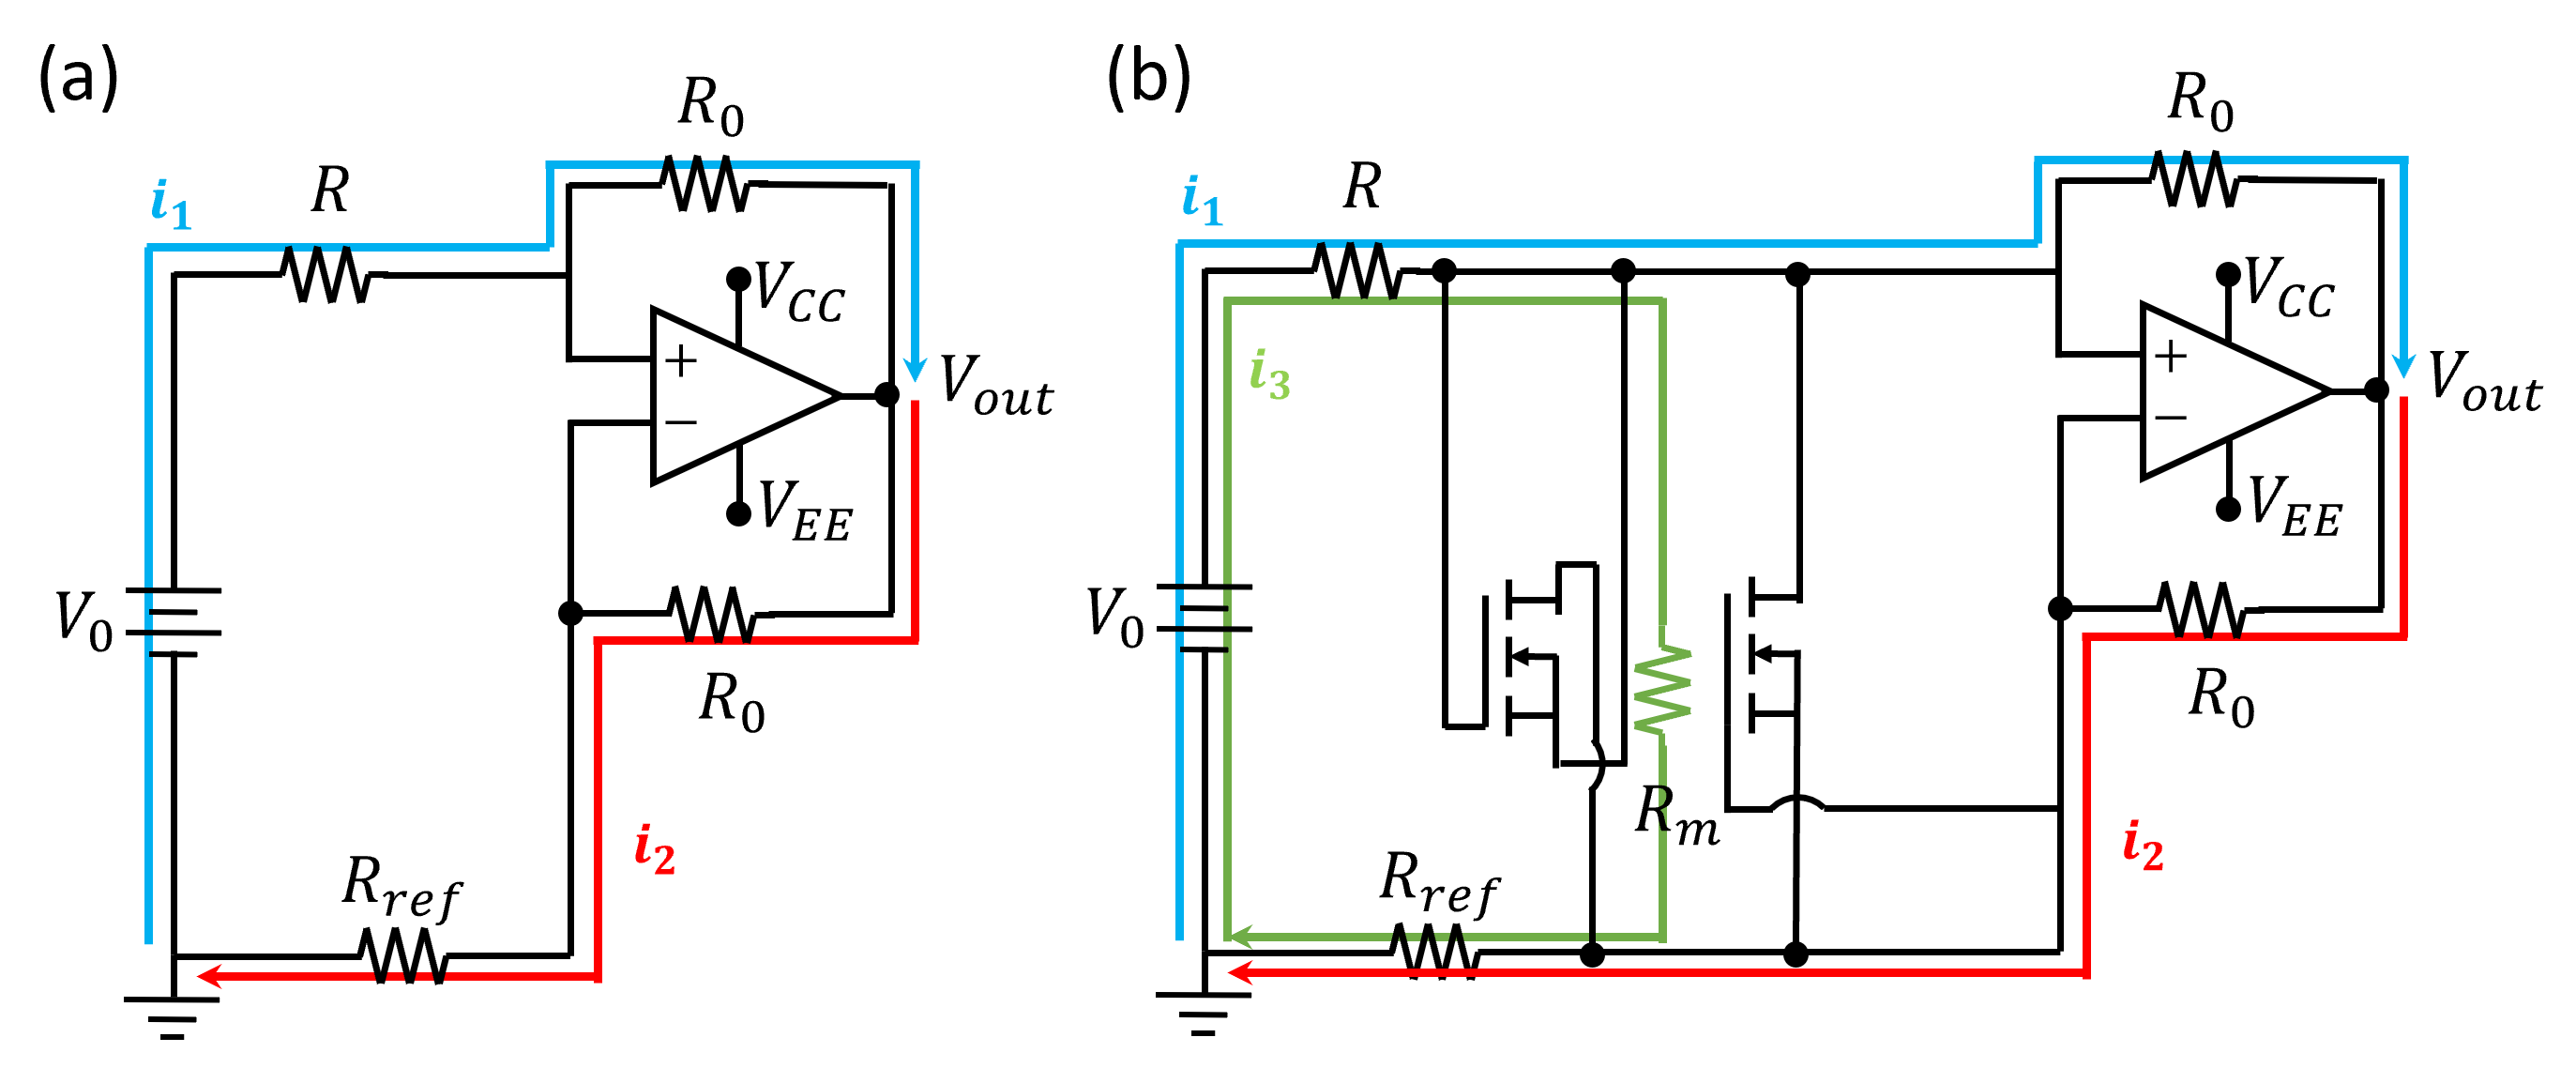
\includegraphics[width=0.45\textwidth]{./figures/TheoryCalc.png}
  \caption{The (a) capacitance and (b) resistance about the normalized deviation of phase difference. }
  \label{fig:stdphiandRC}
\end{figure}

\begin{figure}[!htbp]
  \begin{subfigure}{0.15\textwidth}
    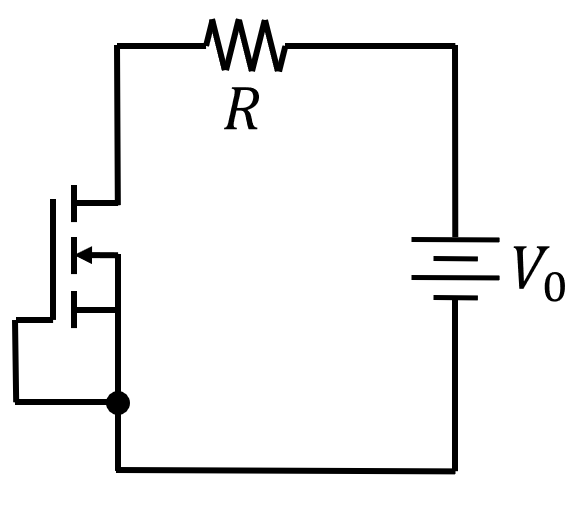
\includegraphics[width=\linewidth]{figures/MOSFET_circuit.png}
    \caption{}
    \label{MOSFET_circuitfig_a}
  \end{subfigure}%
  %\hspace*{\fill}   % maximize separation between the subfigures
  \begin{subfigure}{0.23\textwidth}
    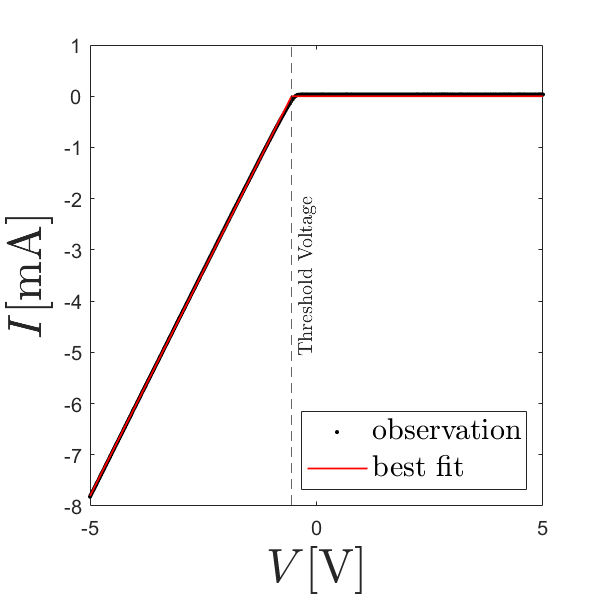
\includegraphics[width=\linewidth]{figures/MOSFETIV.png}
    \caption{}
    \label{MOSFET_circuitfig_b}
  \end{subfigure}

\caption{(a) A schematic setup for testing MOSFET $I-V$ characteristic. (b) Experimental result of MOSFET $I-V$ characteristic. Black dots show experiment data and red line is the best fit to Eq. \ref{MOSFET_eq}. Threshold voltage is denoted as dashed line.} \label{MOSFET_circuitfig}
\end{figure}

In this experiment we used two MOSFETs with gate terminal and source terminal connected each other.
MOSFET is open when the gate--source voltage is higher than the threshold voltage, and current through MOSFET linearly increases as gate--drain voltage increases.
We can characterize this property as 

\begin{equation}
I=\frac{V-V_{\textrm{th}}}{(R+R_{\textrm{MOS}})}\theta(V-V_{\textrm{th}})
\label{MOSFET_eq}
\end{equation}

\noindent where $V_{\textrm{th}}$ is threshold voltage, $R_{\textrm{MOS}}$ is effective resistance of MOSFET, and $\theta(V)$ is Heaviside step function.
To test this $I-V$ characteristic, we set the circuit as Fig. \ref{MOSFET_circuitfig_a}.
We sourced voltage from -5.00V to +5.00V in increments of 0.01V, with a resistor of $R=$560 $\Omega$.
The result is plotted in Fig. \ref{MOSFET_circuitfig_b}, where experimental data is denoted as black dots, best fit to Eq. \ref{MOSFET_eq} as red line, and threshold voltage as dashed line.
Note that the gate--drain voltage is negative when $V_{0}>0$ and vice versa in this setup, so we put $(V-V_{\textrm{th}})\rightarrow-(V-V_{\textrm{th}})$ and $I\rightarrow -I$ into the equation.
Our best fit values are $V_{\textrm{th}}=0.5505\pm0.0015$ V and $R_{\textrm{MOS}}=10.21\pm0.33\>\Omega$.


\section{Derivation of the theoretical $I-V$ Characteristics of the Negative Resistor}
\subsubsection{\label{opampiv}Op-Amp}
For the 

\subsubsection{\label{opamp_mosfetiv}Op-Amp and MOSFETs}
The unsaturated region of the negativer resistor using enabling MOSFETs is identical to the unsaturated region of the negative resistor without the MOSFETs, since all of the MOSFETs do not flow current. We derive a theoretical description of the differential resistance slopes for the region where a MOSFET is opened. 

The three currents present after saturation are depicted in Fig. . In the saturated state, the output voltage of the Op-Amp is fixed as $V_{out}-V_{sat}$. Then the following equations can be obtained.


\begin{equation}
  V_{sat} = V_{in}-R(i_1+i_2)-i_1R_0
\end{equation}
\begin{equation}
  V_{in} - R(i_1+i_2)-R_mi_2-R_{ref}(i_2+i_3) = 0
\end{equation}
\begin{equation}
  V_{sat} -i_3R_0-(i_2+i_3)R_{ref} = 0
\end{equation}

When solving the previous equtions, a solution we can obtain is the following:
\begin{equation}
  i_1 = \frac{V_{sat}(-R_0R_{ref}-R_0R-R_mR_0-R_mR_{ref})+V_{in}(R_0R_{ref}+R_mR_0+R_mR_{ref})}{R_0^2R_{ref}+R_0^2R+R_mR_0^2+2R_0R_{ref}R+eR_0R_{ref}+R_mR_0R+R_mR_{ref}R}
\end{equation}
\begin{equation}
  i_2 = \frac{R_0(V_{sat}(-R_{ref}+R)+V_{in}(R_0+R_{ref}))}{R_0^2R_{ref}+R_0^2R+R_mR_0^2+2R_0R_{ref}R+R_mR_0R_{ref}+R_mR_0R+R_mR_{ref}R}
\end{equation}
\begin{equation}
  i_3 = \frac{V_{sat}(R_0R_{ref}+R_0R+R_mR_0+R_mR)-V_{in}R_0R_{ref}}{R_0^2R_{ref}+R_0^2R+R_mR_0^2+2R_0R_{ref}R+R_mR_0R_{ref}+R_mR_0R+R_mR_{ref}R}
\end{equation}

The current flowing through $R$ is $i_1+i_2$, thus giving the proportional constant to $V_{in}$ as the following:
\begin{equation}
  i_1+i_2 = \frac{R_0R_{ref}+R_0R_m+R_mR_{ref}+R_0^2+R_{ref}R_0}{R_0^2(R_{ref}+R+R_m)+R_0(2R_{ref}R+R_{ref}R_m+R_mR)+R_mR_{ref}R}V_{in} + \text{Intercept}
\end{equation}

\begin{equation}
  V_{in}-Ri_1 = V_+
\end{equation}
\begin{equation}
  V_+ -R_0i_1 = V_{out}
\end{equation}
\begin{equation}
  V_{out}-R_0i_2=V_-
\end{equation}
\begin{equation}
  V_--R_{ref}i_2=0
\end{equation}
\begin{equation}
  V_+ = V_-
\end{equation}
By solving these $5$ equations, the following results can be obtained.
\begin{equation}
  V_{out} = \frac{R_{ref}+R_0}{R_{ref}-R}V_{in}
\end{equation}
\begin{equation}
  i_1 = -\frac{1}{R_{ref}-R}V_{in}
\end{equation}
\end{document}